\documentclass[11pt,twocolumn]{article}
\usepackage{graphicx}
\usepackage{pdfpages}
\usepackage{hyperref}
\usepackage[margin=1.25in]{geometry}
\graphicspath{ {./Figures/} }
\hypersetup{
    colorlinks=true,
    linkcolor=blue,
    filecolor=magenta,      
    urlcolor=cyan,
}
\urlstyle{same}
\usepackage[font={small,it}]{caption}
\usepackage{fancyvrb}
\title{Model \& Simulation of South Bend Government Call Center using Arena}
\author{John D. Bulger, Jacob D. White \& Adali J. J. Johnson, Valparaiso University\thanks{``We have neither given or received, nor have we tolerated other’s use of unauthorized aid."}}
\date{October 2, 2018}
\begin{document}
\maketitle

\section{Introduction (Serving as our Proposal)}
The city of South Bend, located in northern Indiana, established a citizen-accessible call center in February 2013.  It addresses almost every aspect of city-citizen interaction, including waste pick-up and removal, water billing and disconnections, and code enforcement.  By serving as a central hub for communication, the call center is able to consolidate a substantial amount of data regarding citizens as consumers.  This data is available on South Bend's open data portal at \textit{https://data-southbend.opendata.arcgis.com}.

\begin{figure}[h]
	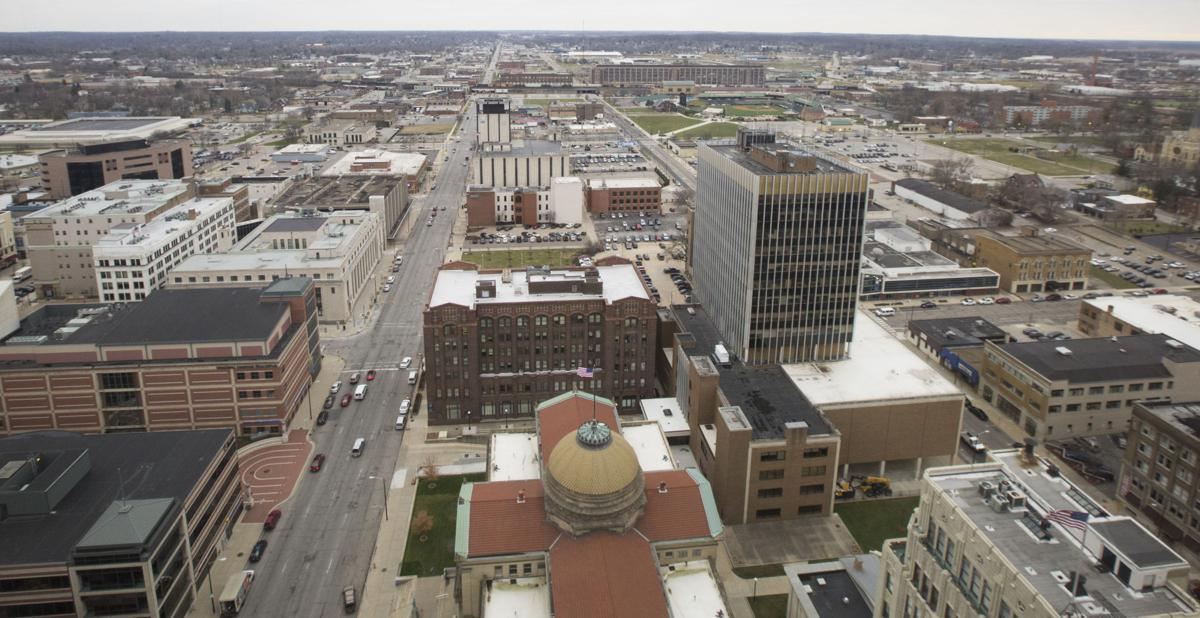
\includegraphics[scale=.17]{south_bend.png}
	\caption{South Bend, IN (Greg Swiercz)}
\end{figure}

\par
The overall purpose of this model is to support decision-making by call center management.  The specific goal of the model is yet to be determined, and will depend on what question the call center poses to us.  In the event this falls through, the model will be built and simulated in order to evaluate the current number of operators.  By exploring this question, the optimal number of operators can be discovered that would keep customer satisfaction (measured in wait time and abandonments) to a specific threshold.  Additionally, the model may be expanded and explored in other directions. One such direction could be determining if operators should have specific topics they handle, as opposed to handling all calls.  Would this make a more effective call center?  Another option could be to model the effect of making certain topics/actions automated, so that the caller never has to interact with an agent.  Simulations of this could determine if it would be beneficial for the call center management to explore such options.
\par
This background data, much of it already organized and cleaned in a preceding analysis, will serve as the basis of this model.  Through the use of this data, assumptions will be minimized as arrival distributions, duration distributions, and operator scheduling can be accurately extrapolated from real data.  Additionally, this model will incorporate the voice-mails left by customers after-hours, that must be returned by the operators throughout the day.  Assumptions will be included, however, that allow for callers to request to be transferred to a supervisor for rare issues and to model customer wait tolerance, along with other yet undetermined interactions.
\par
The basic model structure is based off of the work of Mandelbaun in 2001.  In his work, he lays out the basic schematic of a call center model.\cite{mandelbaun}  This project-specific model will incorporate other avenues and processes, in order to accurately reflect the actual city call center.

\begin{figure}[h]
	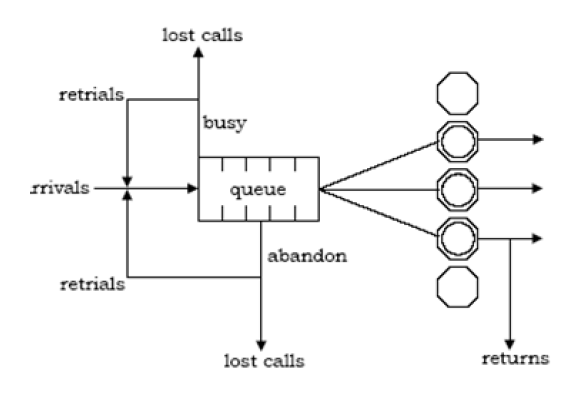
\includegraphics[scale=.45]{call_center_layout.png}
	\caption{Operational Schematic of Call Center (Mandelbaun 2001)}
\end{figure}

A core component of this project will be discovering actual distributions from historical data, even down to the hour of the day.  Although this will present much additional work when compared to assuming distributions, it will create a much more accurate model.  The ultimate goal is to create a successful enough model so that our findings can be communicated to, and hopefully implemented by, the city of South Bend.  The background data analysis will be conducted in Python, and the model will be constructed in Arena.  A rough, simplistic initial thought process of this model can be found on the following page.

\begin{thebibliography}{5}

\bibitem{mandelbaun}
Mandelbaun A., A. Sakov and S. Zeltyn. 2001. Empirical Analysis of a Call Center. Technion Israel Institue of Technology, Israel.

\end{thebibliography}
\newpage
\clearpage
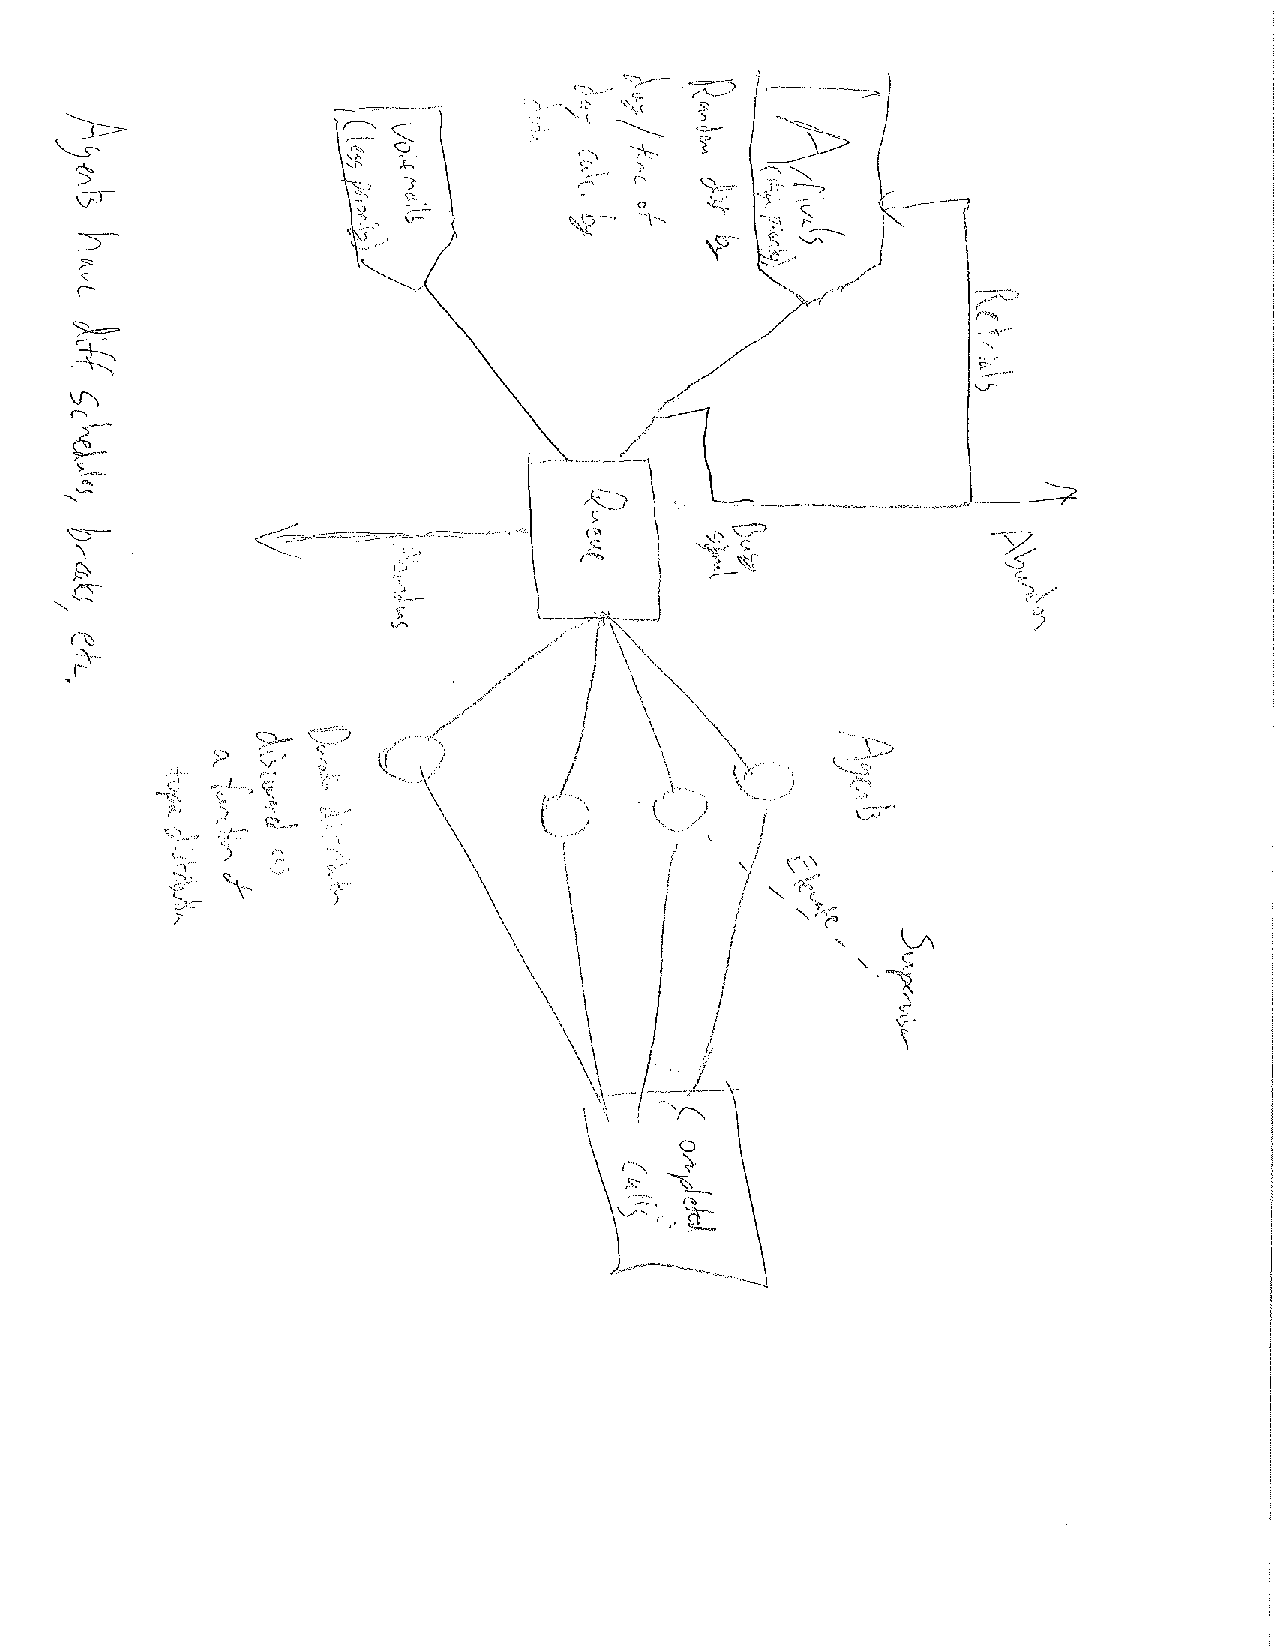
\includepdf{Figures/rough_model_layout}
\end{document}